\title{Comparing Testability and Code Quality in Software Paradigms}
\author{
        Marc Coquand\\
        Department of Computer Science\\
        Umeå University\\
}
\date{\today}


\documentclass[12pt]{article}
\usepackage{listings}
\usepackage{amsthm}
\usepackage[utf8]{inputenc}
\usepackage[english]{babel}
\usepackage{tikz}
\usetikzlibrary{arrows}
\usepackage{float}

\theoremstyle{definition}
\newtheorem*{definition}{Definition}

\theoremstyle{theorem}
\newtheorem*{theorem}{Theorem}

\lstdefinestyle{customc}{
	belowcaptionskip=1\baselineskip,
	breaklines=true,
	frame=L,
	xleftmargin=\parindent,
	language=C,
	showstringspaces=false,
	basicstyle=\footnotesize\ttfamily,
	keywordstyle=\bfseries\color{green!40!black},
	commentstyle=\itshape\color{purple!40!black},
	identifierstyle=\color{blue},
	stringstyle=\color{orange},
}
\lstdefinestyle{customasm}{
	belowcaptionskip=1\baselineskip,
	frame=L,
	xleftmargin=\parindent,
	language=[x86masm]Assembler,
	basicstyle=\footnotesize\ttfamily,
	commentstyle=\itshape\color{purple!40!black},
}
\lstset{escapechar=@,style=customc}

\begin{document}
\maketitle

\begin{abstract} 

    This study's goal is to compare approaches to functional programs and
    object-oriented programs to find how it affects maintainability and code
    quality.  By looking at 3 cases, we analyze, how does a functional approach
    to software architecture compare to an OOP (Object-oriented programming)
    approach when it comes to maintainability and code quality?

\end{abstract}

\section{Introduction}
This is time for all good men to come to the aid of their party!


\section{Theory}\label{theory}

\subsection{Characteristics of Functional Programming}
Expressions and functions

\subsubsection{Iterator pattern}

\subsection{Object Oriented Programming}\label{oop}
Uses variables, commands and procedures

\subsubsection{SOLID principles}

\section{Methods}\label{methods}

\subsection{Cyclomatic Complexity}\label{cyclomaticcomplexity}

Cyclomatic complexity is a complexity measure that looks to control the number
of paths through a program. The Cyclomatic complexity is an upper bound for the number of
test cases required to obtain branch coverage of the code. 

\theoremstyle{definition}
\begin{definition}
The cyclomatic number $v(G)$ of a graph G with $n$ vertices, $e$ edges and $p$
connected components is $v(G) = e - n + p$.
\end{definition}

\begin{theorem}
In a strongly connected graph $G$, the cyclomatic number is equal to the
maximum number of linearly independent circuits.~\cite{McCabe}
\end{theorem}

Informally, we can think of cyclomatic complexity as a way to measure the amount
tests a program needs. The edges of the graph represents the branches caused by
a decision. We do this by creating a graph of the control flow of the program
and calculate each node. If we have the code found in example
figure~\ref{c1excode}.

\begin{figure}[H]
    \begin{lstlisting}
    public static boolean containsLetter(String s) {
      for (int i = 0; i < s.length(); i++) {
        if (Character.isLetter(s.charAt(i))) {
          return true;
        }
      }
      return false;
    }
    \end{lstlisting}
wever 
    \caption{Simple for loop code.}\label{c1excode}
\end{figure}

To calculate the complexity of this function we first construct a graph as seen
in figure~\ref{fig:c1exgraph}. We find that the cyclomatic number is 3.
\begin{figure}[H]
    \centering
    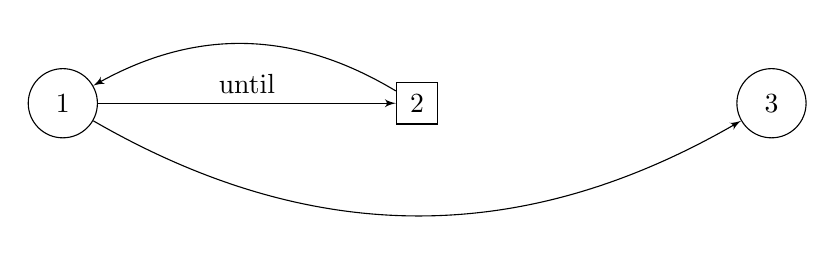
\begin{tikzpicture}
        \tikzset{vertex/.style = {shape=circle,draw,minimum size=2.5em}};
        \tikzset{edge/.style = {->,> = latex'}};
        \node[vertex] (a1) at (1.5,0) {1};
        \node[shape=rectangle,draw,minimum size=1.5em] (a2) at (6,0) {2};
        \node[vertex] (a3) at (10.5,0) {3};
        \draw[edge] (a2)  to[bend right]  (a1);
        \draw[edge] (a1) to node[above]{until} (a2) ;
        \draw[edge] (a1) to[bend right] (a3);
    \end{tikzpicture}
    \caption{Cyclomatic complexity graph for figure~\ref{c1excode}}\label{fig:c1exgraph}
\end{figure}

\subsubsection{Cyclomatic Complexity in Functional Programming}

The definition of cyclomatic complexity in Section~\ref{cyclomaticcomplexity} is
not ideal for functional programming. Cyclomatic complexity is calculated by
creating graphs based on control flow operations such as while loops and if
statements. In functional programming everything is a function, thus the
cyclomatic complexity will always tend to 0 using this definition. Thus we will
define a different method of calculating the cyclomatic complexity for
functional programs.~\cite{bergklaas}

\subsection{Cognitive Dimensions}

\subsection{Case studies}

\subsubsection{Simplified chess game}

Chess is a famous game and assumed that the reader know how it works. Aim
is to implement a simplified variant of it. This is not ordinary chess but a
simplified version:

\begin{itemize} 
    \item Only pawns and horses exist.
    \item You win by removing all the other players pieces.
\end{itemize}

The player should be able to do the following:

\begin{itemize} 
    \item List all available moves for a certain chess piece. 
    \item Move the chess piece to a given space
    \item Switch player after move
    \item Get an overview of the board
    \item Get an error when making invalid moves
\end{itemize}

\subsubsection{to-do List}

A common task in programming is to create some kind of data store with
information. A to-do list is a minimal example of that. It consists of a list of
items that can be used to remember what to do later. The user should be able to:

\begin{itemize}
    \item Create a new item in the to-do list.
    \item Remove an item from the to-do list.
    \item See all items in the to-do list.
    \item Update an item from the to-do list.
\end{itemize}

\subsubsection{Chatbot engine}

Oftentimes when developing applications we have to deal with complex information
input. One of those cases is when we have chat bots. Chat bots are interactive
programs that respond with a text answer to the users input. For this
application we will implement the following:

\begin{itemize}
    \item Interpretor that can handle semi-complex inputs and deal with errors.
    \item Give answers to those inputs in form of text messages.
\end{itemize}    

\section{Results}\label{results}

\section{Conclusions}\label{conclusions}

\section{Limitations}\label{limitations}

\subsection{Improvements to implementation}

\bibliographystyle{abbrv}
\bibliography{thesis}

\end{document}
